\documentclass[tikz]{standalone}
\usetikzlibrary{arrows.meta,
                chains,
                positioning,
                shapes.geometric
                }
% for fancy looks of data storages
\begin{document}
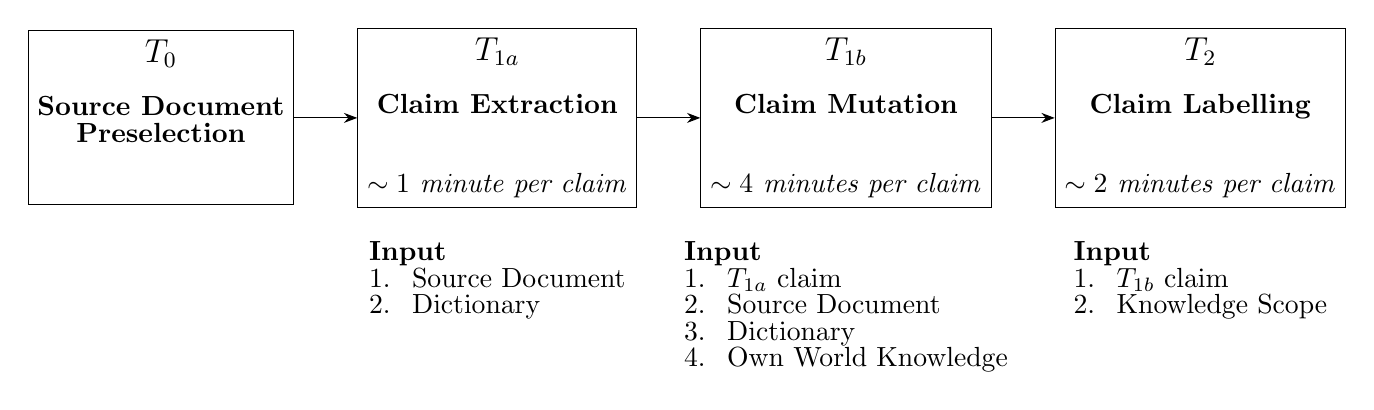
\begin{tikzpicture}[
        node distance = 3mm and 8mm,
        start chain = going right,
        mdl/.style = {shape=ellipse, aspect=2.2, draw},
        task/.style = {draw, align=center, font=\linespread{0.8}\selectfont},
        input/.style = {align=left, font=\linespread{0.8}\selectfont}
    ]
    \begin{scope}[every node/.append style={on chain, join=by -Stealth}]
        \node (t0) [task] {
            \large{$T_0$}\\\\
            \textbf{Source Document}\\
            \textbf{Preselection}\\\\
        };
        \node (t1a) [task]  {
            \large{$T_{1a}$}\\\\
            \textbf{Claim Extraction}\\\\\\
            \textit{$\sim 1$ minute per claim}
        };
        \node (t1b) [task]  {
            \large{$T_{1b}$}\\\\
            \textbf{Claim Mutation}\\\\\\
            \textit{$\sim 4$ minutes per claim}
        };
        \node (t2) [task]  {
            \large{$T_2$}\\\\
            \textbf{Claim Labelling}\\\\\\
            \textit{$\sim 2$ minutes per claim}
        };
    \end{scope}
    \node[input,below=of t1a]  {
        \textbf{Input}\\
        1.~ Source Document\\
        2.~ Dictionary
    };
    \node[input,below=of t1b]  {
        \textbf{Input}\\
        1.~ $T_{1a}$ claim\\
        2.~ Source Document\\
        3.~ Dictionary\\
        4.~ Own World Knowledge
    };
    \node[input,below=of t2]  {
        \textbf{Input}\\
        1.~ $T_{1b}$ claim\\
        2.~ Knowledge Scope
    };
\end{tikzpicture}
\end{document}